\subsection{Receiver Side (RTC Reconstruction Pipeline)}

\vspace{0.25cm}

\begin{figure}[H]
    \centering
    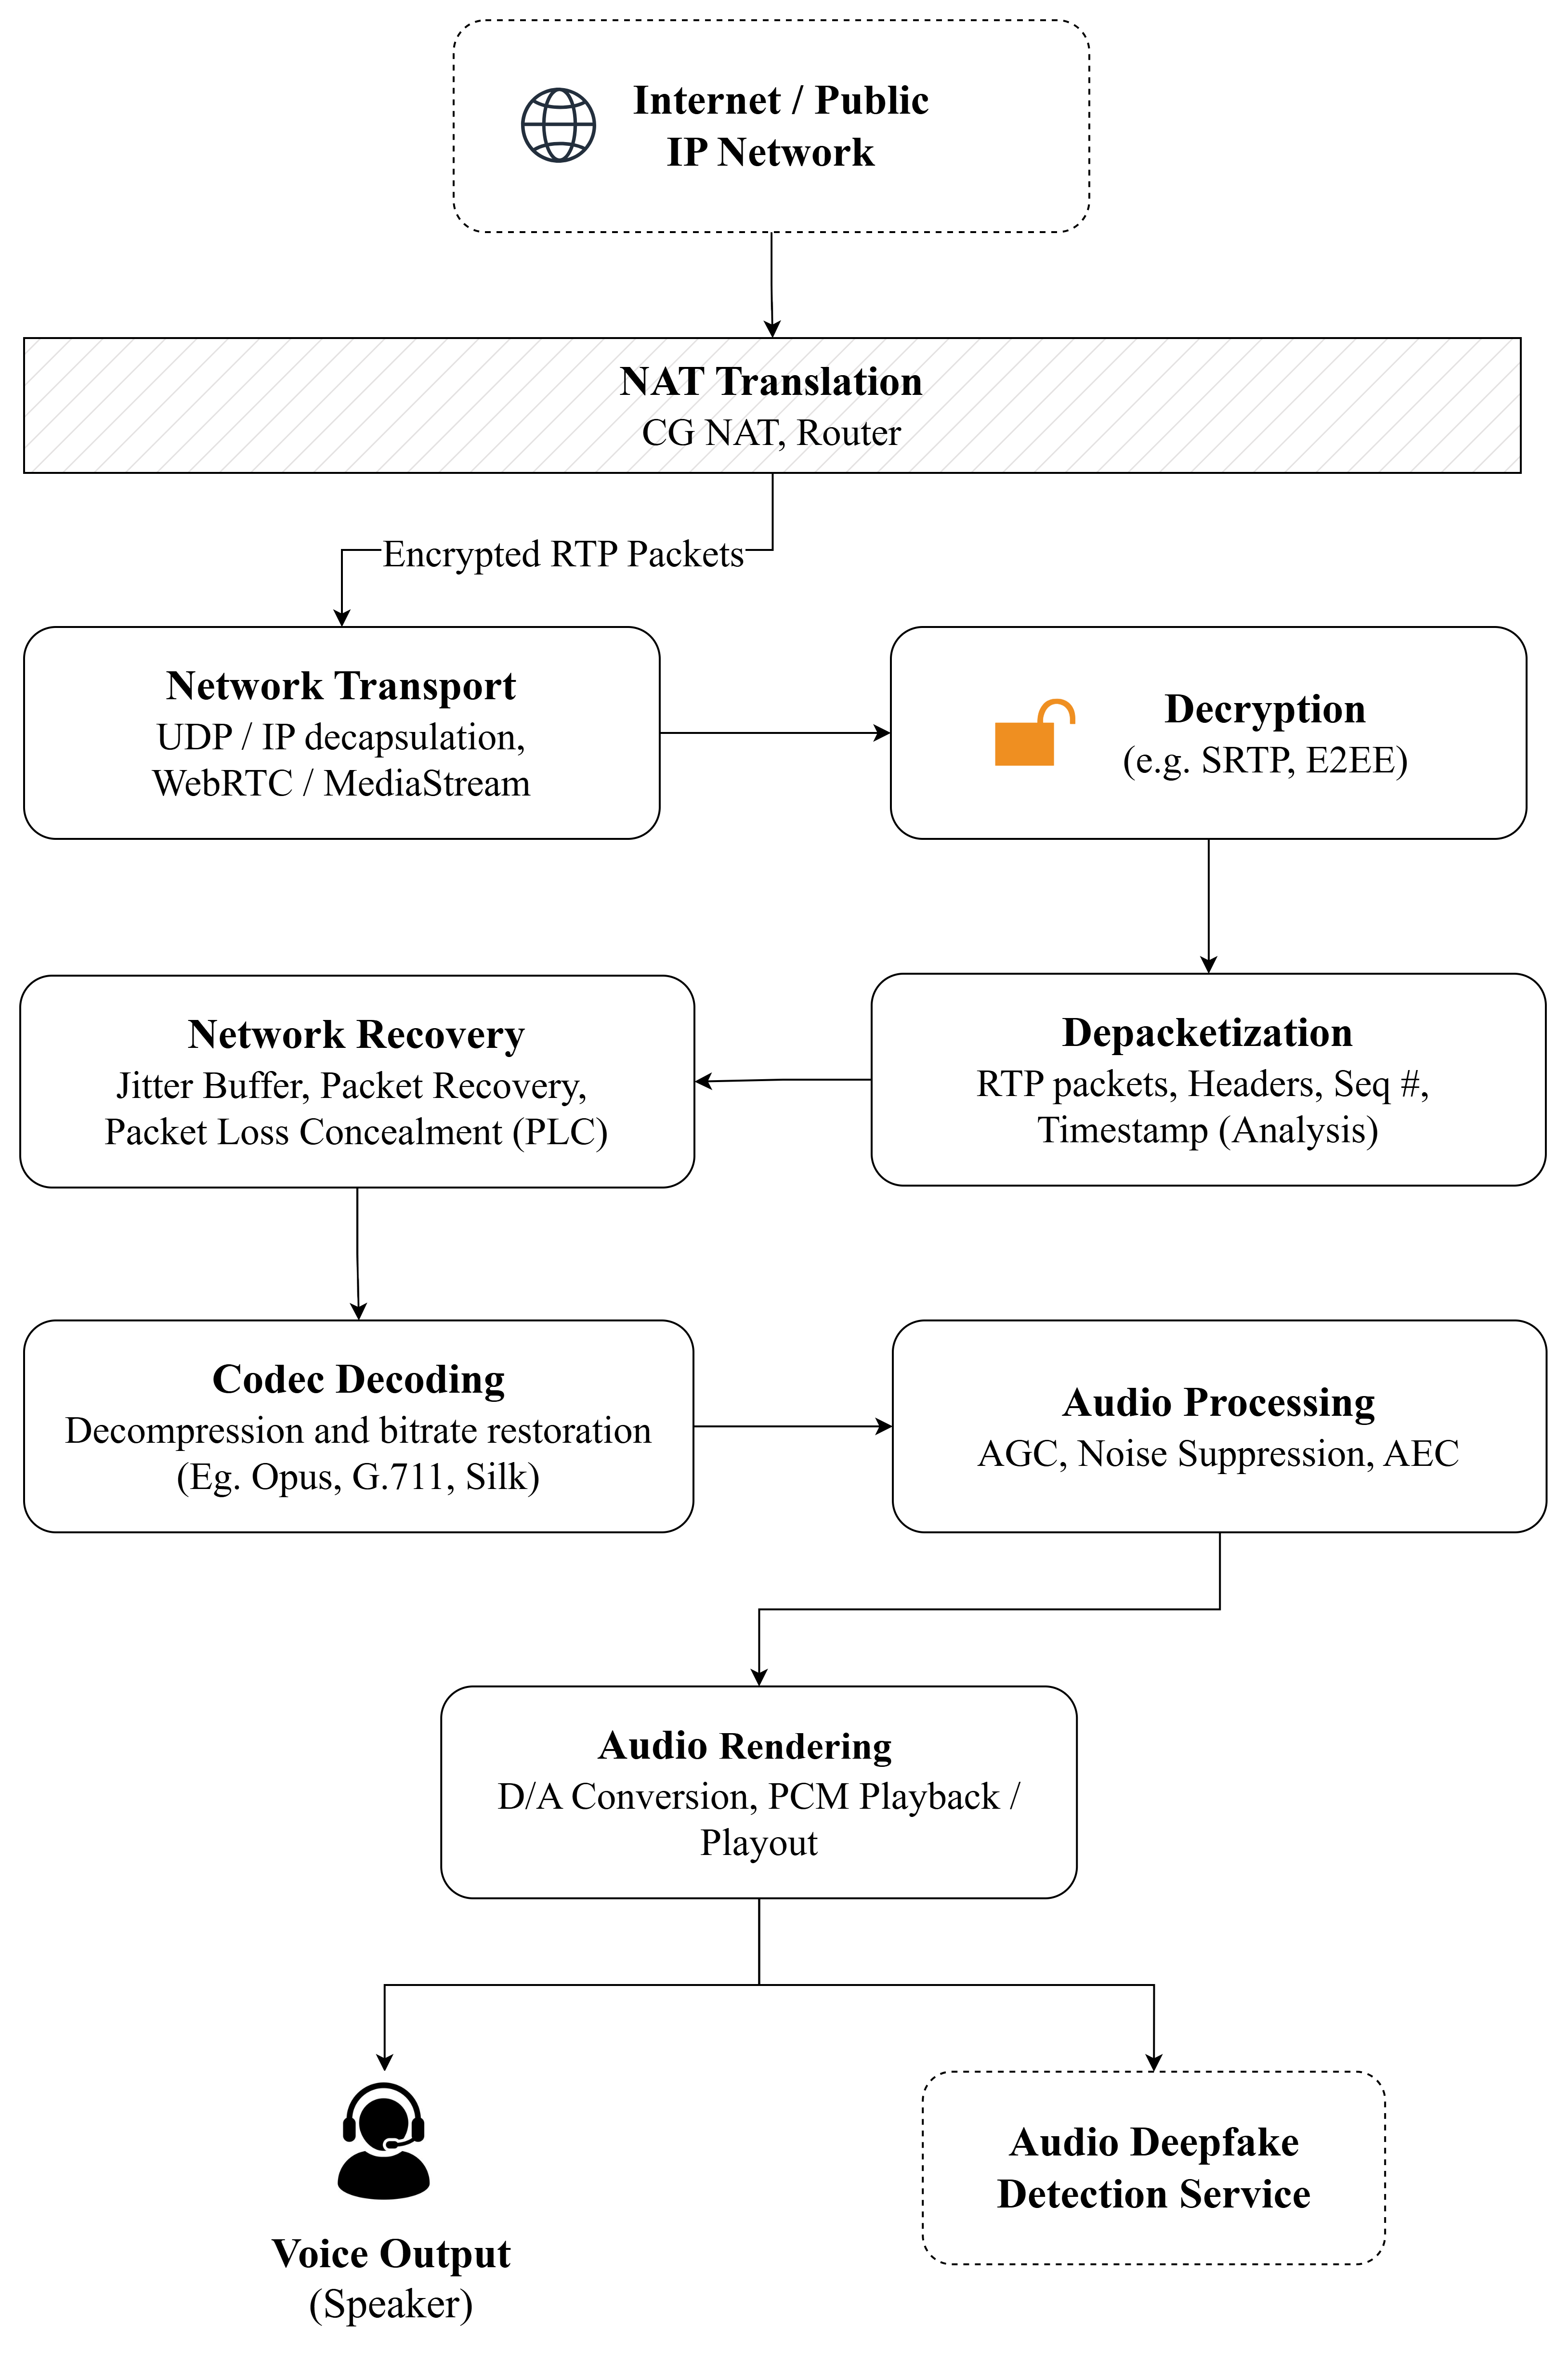
\includegraphics[width=1\textwidth]{images/methodology/receiver_side.png}
    \caption{Receiver-side RTC Reconstruction Pipeline}
    \label{fig:receiver_side}
\end{figure}

The receiver side represents the reconstruction stage of the RTC system, where incoming network packets are converted back into a continuous audio stream for playback or downstream processing. This stage is critical because it produces the actual signal observed by the proposed deepfake detection service. In practical RTC deployments, the received signal is not a clean reconstruction of the original waveform; rather, it is a transformed version shaped by network impairments, packet handling mechanisms, codec decoding, and receiver-side enhancement operations.

In the proposed framework, the receiver pipeline is treated as a realistic reconstruction module that reflects the behavior of deployed VoIP and RTC systems. The output of this stage defines the input domain for the detection service, and therefore its distortions must be modeled carefully.

\subsubsection{Packet Reception and Ordering}

At the receiver, incoming audio packets are collected from the transport layer and processed in the order required for stream reconstruction. Due to network variability, packets may arrive out of order, delayed, duplicated, or missing.

Let the transmitted packet sequence be represented as
\begin{equation}
P_t = \{p_1, p_2, \ldots, p_n\},
\end{equation}
and let the set of packets successfully received at the destination be
\begin{equation}
P_r = \{p_1^{(r)}, p_2^{(r)}, \ldots, p_m^{(r)}\}, \quad m \leq n.
\end{equation}
Here, \(p_i^{(r)}\) denotes the received version of packet \(p_i\). Sequence numbers and timestamps are used to detect packet loss and restore the correct temporal ordering of the stream.

The packet reception stage therefore performs the following operations:
\begin{itemize}
    \item collection of arriving packets from the network stack,
    \item detection of missing or delayed packets using sequence identifiers,
    \item reordering of packets according to timestamps,
    \item preparation of packets for buffering and decoding.
\end{itemize}

Perfect reconstruction is not guaranteed when packet loss, delay variation, or reordering occurs.

\subsubsection{Packet Authentication and Decryption}

Received packets are first subjected to integrity verification to ensure that they have not been modified during transmission. Following successful verification, the encrypted payload is decrypted using the session keys established during call setup.

This process restores the original compressed audio data while maintaining confidentiality and protection against unauthorized access.

\subsubsection{Depacketization}

After decryption, the Real-Time Transport Protocol (RTP) headers are analyzed. Sequence numbers and timestamps contained within the packet headers provide information about packet ordering and playback timing.

These metadata fields enable the receiver to identify missing packets, detect out-of-order arrivals, and reconstruct the original audio sequence.

\subsubsection{Jitter Buffer and Stream Stabilization}

Since packets may arrive with irregular timing, RTC systems typically employ a jitter buffer to stabilize playback. The jitter buffer temporarily stores incoming packets and releases them at a controlled rate so that the downstream decoder receives a more regular stream.

The jitter buffer serves three main purposes:
\begin{itemize}
    \item compensating for variation in packet arrival times,
    \item reordering packets before decoding,
    \item maintaining continuous audio playback with minimal interruptions.
\end{itemize}

However, this stabilization comes at the cost of additional delay and possible temporal modification of the signal. When network jitter is severe, the buffer may drop late packets or duplicate previous frames to preserve continuity. This causes buffer output to temporally smoothed but not signal-faithful. This behavior is particularly important in deepfake detection because fine-grained temporal artifacts may be attenuated or altered by buffering operations.

\subsubsection{Packet Loss Concealment}

When packets are missing or arrive too late for playout, the receiver applies packet loss concealment (PLC) to generate a plausible replacement for the missing audio frame. PLC is commonly implemented using waveform repetition, interpolation, predictive synthesis, or codec-specific concealment strategies.

Let the buffered packet stream be represented as \(P_b\). The concealment process can be expressed as
$P_b \rightarrow P_c,$
where \(P_c\) denotes the packet stream after missing frames have been concealed.

Although PLC improves perceptual continuity, it also introduces synthetic artifacts and may smooth over abrupt acoustic transitions. These modifications can partially mask the characteristics that are relevant for deepfake detection. PLC does not recover the original missing content; it only generates a perceptually acceptable approximation.

\subsubsection{Audio Decoding Process}

After buffering and concealment, the compressed payloads are passed to the codec decoder to reconstruct waveform samples. The decoder transformation can be modeled as

\begin{equation}
\hat{x}[n] = D(x_c),
\end{equation}

where $x_c$ denotes the compressed bitstream and $\hat{x}[n]$ represents the reconstructed discrete-time speech signal.

The characteristics of the reconstructed signal depend on the codec employed during transmission:

\begin{itemize}
\item \textbf{Opus:} The most widely used codec in modern RTC systems. Opus combines linear prediction and transform-based coding techniques with adaptive bitrate control. During decoding, quantization artifacts, spectral smoothing, bandwidth limitations, and temporal distortions may be introduced, particularly under low-bitrate operating conditions.

\item \textbf{G.711:} A waveform-based codec commonly used in traditional telephony systems. Decoding primarily involves inverse companding, resulting in relatively low algorithmic distortion but offering limited bandwidth efficiency compared to modern codecs.

\item \textbf{AAC:} A transform-domain codec that employs perceptual audio coding techniques. Reconstruction may introduce quantization noise and perceptual smoothing effects, particularly in high-frequency regions of the spectrum.

\end{itemize}

In general, decoding is not a lossless process. Even under ideal network conditions, codec reconstruction introduces approximation errors due to compression and quantization. Consequently, the reconstructed signal preserves speech intelligibility while potentially altering fine-grained acoustic characteristics that may be relevant for deepfake detection. 

\subsubsection{Receiver-Side Audio Enhancement}

After decoding, RTC systems often apply additional enhancement operations to improve perceptual quality. These operations are implementation-dependent but typically include automatic gain control, noise suppression, and acoustic echo cancellation.

Let the decoded signal be \(\hat{x}[n]\). The receiver-side enhancement pipeline can be represented as
\begin{equation}
x_{rtc}[n] = T_{rtc}(\hat{x}[n]),
\end{equation}
where \(T_{rtc}(\cdot)\) denotes the combined receiver-side processing chain and \(x_{rtc}[n]\) is the final reconstructed RTC audio signal.

Common enhancement modules include:
\begin{itemize}
    \item \textbf{Automatic Gain Control (AGC):} normalizes signal amplitude to maintain consistent loudness,
    \item \textbf{Noise Suppression:} reduces stationary and non-stationary background noise,
    \item \textbf{Echo Cancellation:} suppresses feedback caused by speaker-to-microphone acoustic coupling.
\end{itemize}

These modules improve usability in real-time communication but can also alter amplitude dynamics, harmonic structure, and low-energy components of the speech signal. Such transformations are relevant because deepfake artifacts may be partially suppressed or distorted by receiver-side enhancement.

\subsubsection{Output Signal for Deepfake Detection}

The final output of the receiver pipeline is the audio stream presented to the proposed deepfake detection service. This signal represents the actual deployment-domain input rather than pristine source audio.

The overall receiver-side transformation may be summarized as
\begin{equation}
x_{out}[n] = \mathcal{T}_{rtc}\!\left(\mathcal{T}_{net}\!\left(C(x[n])\right)\right),
\end{equation}
where
\begin{itemize}
    \item \(x[n]\) is the input audio waveform at the sender side,
    \item \(C(\cdot)\) denotes codec compression and reconstruction,
    \item \(\mathcal{T}_{net}(\cdot)\) denotes network-induced distortions,
    \item \(\mathcal{T}_{rtc}(\cdot)\) denotes receiver-side buffering, concealment, and enhancement operations,
    \item \(x_{out}[n]\) is the final reconstructed signal used for analysis.
\end{itemize}

The output audio is therefore temporally stabilized, perceptually enhanced, and potentially distorted by multiple stages of processing. This makes receiver-side modeling essential for evaluating deepfake detection under realistic RTC conditions.